% core_register_placement.tex -- every register (flip-flop) of the 4x4 accelerator core (mm_core),
% drawn inside the block that owns it: 16 PEs, skew buffers A and B, controller FSM, mm_regs, rd_valid.
% Facts come from rtl/core/*.sv with N = 4, K_MAX = 64.
% Build:  tectonic core_register_placement.tex      (or: pdflatex core_register_placement.tex)
% PNG:    pdftoppm -png -r 220 -singlefile core_register_placement.pdf core_register_placement
\documentclass[tikz,border=14pt,12pt]{standalone}
\usepackage[T1]{fontenc}
\usepackage[scaled=0.95]{helvet}
\renewcommand{\familydefault}{\sfdefault}
\usepackage{booktabs}
\usepackage{amsmath}
\usetikzlibrary{arrows.meta,calc}

% ---------------- palette (same as the slide decks) ----------------
\definecolor{pcb}{HTML}{0B2E33}
\definecolor{pcbmid}{HTML}{1F5C61}
\definecolor{tint}{HTML}{E6F0EF}
\definecolor{copper}{HTML}{B5651D}
\definecolor{coppert}{HTML}{F6E8DC}
\definecolor{ink}{HTML}{1F2A2E}
\definecolor{muted}{HTML}{5B6B70}
\definecolor{hardf}{HTML}{DCE6F2}
\definecolor{harde}{HTML}{2F4A7A}
% one colour per register owner: fill / border
\definecolor{pef}{HTML}{8CC7BF}  \definecolor{ped}{HTML}{0B2E33}
\definecolor{skf}{HTML}{BFE3B4}  \definecolor{skd}{HTML}{2E7D32}
\definecolor{ctf}{HTML}{D7C8F0}  \definecolor{ctd}{HTML}{5E3A8C}
\definecolor{rgf}{HTML}{F5C6DF}  \definecolor{rgd}{HTML}{8E2463}
\definecolor{rvf}{HTML}{FFD95E}  \definecolor{rvd}{HTML}{8A6800}
\definecolor{gone}{HTML}{9E9E9E}

\tikzset{
  ffpe/.style   ={draw=ped, fill=pef, line width=0.35pt},
  ffsk/.style   ={draw=skd, fill=skf, line width=0.35pt},
  ffct/.style   ={draw=ctd, fill=ctf, line width=0.35pt},
  ffrg/.style   ={draw=rgd, fill=rgf, line width=0.35pt},
  ffrv/.style   ={draw=rvd, fill=rvf, line width=0.5pt},
  ffgone/.style ={draw=gone, fill=white, densely dashed, line width=0.35pt},
  ffmaybe/.style={draw=rgd, fill=white, densely dotted, line width=0.5pt},
  comb/.style   ={draw=copper, fill=coppert, rounded corners=2pt, thick},
  hard/.style   ={draw=harde, fill=hardf, thick, dashed},
  owner/.style  ={draw=#1, rounded corners=6pt, line width=1.2pt},
  dat/.style    ={-{Stealth[length=1.8mm]}, thick, pcbmid},
  ctl/.style    ={-{Stealth[length=2mm]}, densely dashed, thick, muted},
  lab/.style    ={font=\tiny, text=muted, inner sep=1pt},
  hdr/.style    ={font=\footnotesize\bfseries, text=ink, inner sep=1pt},
}

% \ffrow{x}{y}{n}{cell}{style}: one register of n flip-flops in a row, bottom-left corner at (x,y)
\newcommand{\ffrow}[5]{\foreach \q in {1,...,#3}{\draw[#5] ({#1+(\q-1)*#4},{#2}) rectangle ++(#4,#4);}}
% \ffcol{x}{y}{n}{cell}{style}: one register of n flip-flops in a column, top-left corner at (x,y)
\newcommand{\ffcol}[5]{\foreach \q in {1,...,#3}{\draw[#5] ({#1},{#2-\q*#4}) rectangle ++(#4,#4);}}
% \regname{y}{name}{role}: register name + role in the left column of mm_regs / controller
\newcommand{\regname}[3]{%
  \node[anchor=west, font=\scriptsize, inner sep=0pt] at (0.75,#1+0.2) {#2};
  \node[anchor=west, lab, inner sep=0pt] at (0.75,#1-0.12) {#3};}
\newcommand{\rn}[1]{\texttt{#1}}

\begin{document}
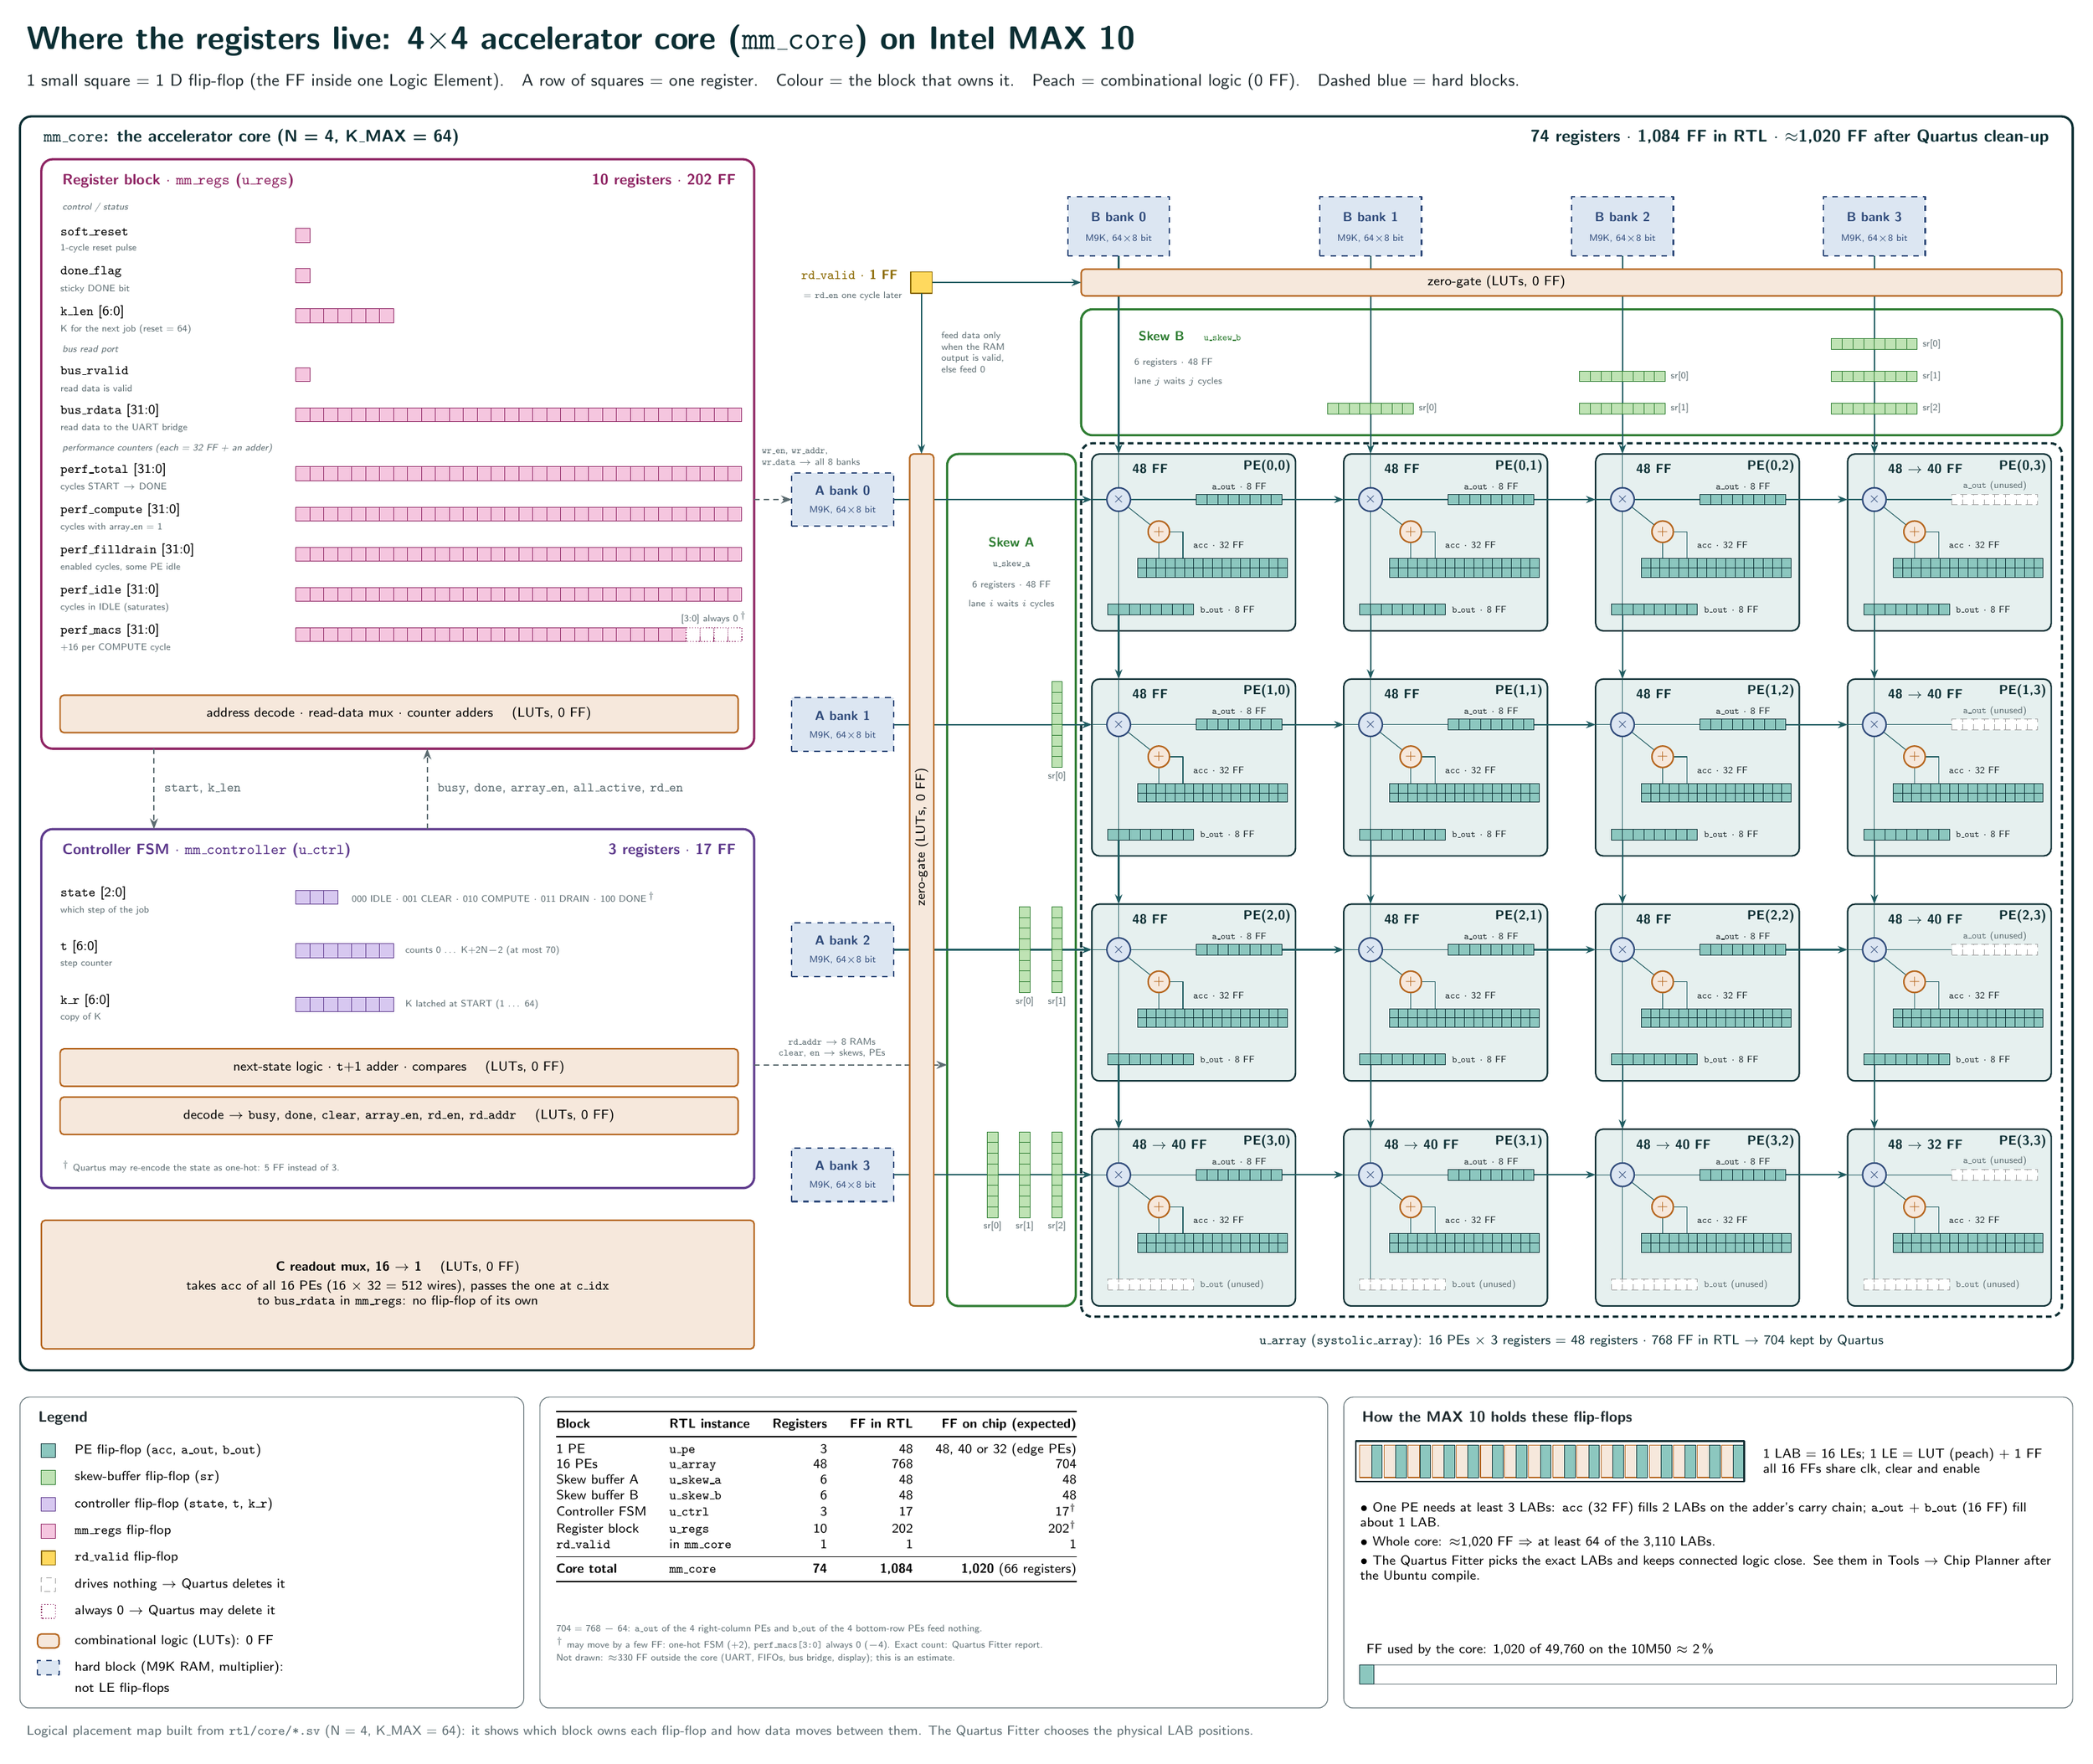
\begin{tikzpicture}[line join=round]

% =====================================================================
% title
% =====================================================================
\node[anchor=west, font=\LARGE\bfseries, text=pcb] at (0,31.1)
  {Where the registers live: 4$\times$4 accelerator core (\rn{mm\_core}) on Intel MAX 10};
\node[anchor=west, font=\small, text=ink] at (0,30.35)
  {1 small square = 1 D flip-flop (the FF inside one Logic Element).\quad
   A row of squares = one register.\quad Colour = the block that owns it.\quad
   Peach = combinational logic (0 FF).\quad Dashed blue = hard blocks.};

% =====================================================================
% owner outlines
% =====================================================================
\draw[owner=pcb] (0,6.3) rectangle (38.3,29.7);
\node[anchor=west, hdr, font=\small\bfseries, text=pcb] at (0.4,29.3)
  {\rn{mm\_core}: the accelerator core (N = 4, K\_MAX = 64)};
\node[anchor=east, hdr, font=\small\bfseries, text=pcb] at (37.9,29.3)
  {74 registers $\cdot$ 1,084 FF in RTL $\cdot$ $\approx$1,020 FF after Quartus clean-up};

\draw[owner=rgd, fill=white] (0.4,17.9) rectangle (13.7,28.9);   % mm_regs
\draw[owner=ctd, fill=white] (0.4,9.7)  rectangle (13.7,16.4);   % controller
\draw[owner=skd] (17.3,7.5)  rectangle (19.7,23.4);              % skew A
\draw[owner=skd] (19.8,23.75) rectangle (38.1,26.1);             % skew B
\draw[owner=ped, densely dashed] (19.8,7.3) rectangle (38.1,23.6); % array

% =====================================================================
% mm_regs : 10 registers, 202 FF
% =====================================================================
\node[anchor=west, hdr, text=rgd] at (0.75,28.5) {Register block $\cdot$ \rn{mm\_regs} (\rn{u\_regs})};
\node[anchor=east, hdr, text=rgd] at (13.4,28.5) {10 registers $\cdot$ 202 FF};

\node[anchor=west, lab, font=\tiny\itshape] at (0.75,28.0) {control / status};
\regname{27.35}{\rn{soft\_reset}}{1-cycle reset pulse}          \ffrow{5.15}{27.35}{1}{0.26}{ffrg}
\regname{26.6}{\rn{done\_flag}}{sticky DONE bit}               \ffrow{5.15}{26.6}{1}{0.26}{ffrg}
\regname{25.85}{\rn{k\_len} [6:0]}{K for the next job (reset = 64)} \ffrow{5.15}{25.85}{7}{0.26}{ffrg}

\node[anchor=west, lab, font=\tiny\itshape] at (0.75,25.35) {bus read port};
\regname{24.75}{\rn{bus\_rvalid}}{read data is valid}           \ffrow{5.15}{24.75}{1}{0.26}{ffrg}
\regname{24.0}{\rn{bus\_rdata} [31:0]}{read data to the UART bridge} \ffrow{5.15}{24.0}{32}{0.26}{ffrg}

\node[anchor=west, lab, font=\tiny\itshape] at (0.75,23.5) {performance counters (each = 32 FF + an adder)};
\regname{22.9}{\rn{perf\_total} [31:0]}{cycles START $\rightarrow$ DONE}   \ffrow{5.15}{22.9}{32}{0.26}{ffrg}
\regname{22.15}{\rn{perf\_compute} [31:0]}{cycles with array\_en = 1}      \ffrow{5.15}{22.15}{32}{0.26}{ffrg}
\regname{21.4}{\rn{perf\_filldrain} [31:0]}{enabled cycles, some PE idle}  \ffrow{5.15}{21.4}{32}{0.26}{ffrg}
\regname{20.65}{\rn{perf\_idle} [31:0]}{cycles in IDLE (saturates)}       \ffrow{5.15}{20.65}{32}{0.26}{ffrg}
\regname{19.9}{\rn{perf\_macs} [31:0]}{+16 per COMPUTE cycle}             \ffrow{5.15}{19.9}{28}{0.26}{ffrg}
\ffrow{12.43}{19.9}{4}{0.26}{ffmaybe}
\node[lab, anchor=south] at (12.95,20.18) {[3:0] always 0\,$^\dagger$};

\draw[comb] (0.75,18.2) rectangle (13.4,18.9);
\node[font=\scriptsize] at (7.07,18.55) {address decode $\cdot$ read-data mux $\cdot$ counter adders \quad (LUTs, 0 FF)};

% mm_regs <-> controller
\draw[ctl] (2.5,17.9) -- (2.5,16.4);
\node[lab, anchor=west, font=\scriptsize] at (2.65,17.15) {\rn{start}, \rn{k\_len}};
\draw[ctl] (7.6,16.4) -- (7.6,17.9);
\node[lab, anchor=west, font=\scriptsize] at (7.75,17.15) {\rn{busy}, \rn{done}, \rn{array\_en}, \rn{all\_active}, \rn{rd\_en}};

% =====================================================================
% controller : 3 registers, 17 FF
% =====================================================================
\node[anchor=west, hdr, text=ctd] at (0.75,16.0) {Controller FSM $\cdot$ \rn{mm\_controller} (\rn{u\_ctrl})};
\node[anchor=east, hdr, text=ctd] at (13.4,16.0) {3 registers $\cdot$ 17 FF};

\regname{15.0}{\rn{state} [2:0]}{which step of the job}  \ffrow{5.15}{15.0}{3}{0.26}{ffct}
\node[lab, anchor=west] at (6.15,15.13) {000 IDLE $\cdot$ 001 CLEAR $\cdot$ 010 COMPUTE $\cdot$ 011 DRAIN $\cdot$ 100 DONE\,$^\dagger$};
\regname{14.0}{\rn{t} [6:0]}{step counter}              \ffrow{5.15}{14.0}{7}{0.26}{ffct}
\node[lab, anchor=west] at (7.15,14.13) {counts 0 \ldots\ K+2N$-$2 (at most 70)};
\regname{13.0}{\rn{k\_r} [6:0]}{copy of K}               \ffrow{5.15}{13.0}{7}{0.26}{ffct}
\node[lab, anchor=west] at (7.15,13.13) {K latched at START (1 \ldots\ 64)};

\draw[comb] (0.75,11.6) rectangle (13.4,12.3);
\node[font=\scriptsize] at (7.07,11.95) {next-state logic $\cdot$ \rn{t}+1 adder $\cdot$ compares \quad (LUTs, 0 FF)};
\draw[comb] (0.75,10.7) rectangle (13.4,11.4);
\node[font=\scriptsize] at (7.07,11.05) {decode $\rightarrow$ \rn{busy}, \rn{done}, \rn{clear}, \rn{array\_en}, \rn{rd\_en}, \rn{rd\_addr} \quad (LUTs, 0 FF)};
\node[lab, anchor=west] at (0.75,10.1) {$^\dagger$ Quartus may re-encode the state as one-hot: 5 FF instead of 3.};

% controller -> datapath
\draw[ctl] (13.7,12.0) -- (17.3,12.0);
\node[lab, anchor=south, align=center] at (15.15,12.1) {\rn{rd\_addr} $\rightarrow$ 8 RAMs\\\rn{clear}, \rn{en} $\rightarrow$ skews, PEs};

% =====================================================================
% C readout mux (combinational, 0 FF)
% =====================================================================
\draw[comb] (0.4,6.7) rectangle (13.7,9.1);
\node[font=\scriptsize, align=center] at (7.05,7.9)
  {\textbf{C readout mux, 16 $\rightarrow$ 1} \quad (LUTs, 0 FF)\\[2pt]
   takes \rn{acc} of all 16 PEs (16 $\times$ 32 = 512 wires), passes the one at \rn{c\_idx}\\
   to \rn{bus\_rdata} in \rn{mm\_regs}: no flip-flop of its own};

% =====================================================================
% datapath geometry
%   PE(i,j): bottom-left (20+4.7j, 20.1-4.2i), size 3.8 x 3.3
%   row i a-lane at y = 22.55-4.2i,  column j b-lane at x = 20.5+4.7j
% =====================================================================

% ---- lanes (drawn first, registers sit on top) ----
\foreach \i in {0,...,3}{
  \pgfmathsetmacro{\ya}{22.55-4.2*\i}
  \draw[dat] (16.3,\ya) -- (20.0,\ya);
}
\foreach \j in {0,...,3}{
  \pgfmathsetmacro{\xb}{20.5+4.7*\j}
  \draw[dat] (\xb,27.1) -- (\xb,23.4);
}

% ---- RAM banks (M9K, not LE flip-flops) ----
\foreach \i in {0,...,3}{
  \pgfmathsetmacro{\ya}{22.55-4.2*\i}
  \draw[hard] (14.4,\ya-0.5) rectangle (16.3,\ya+0.5);
  \node[font=\scriptsize\bfseries, text=harde] at (15.35,\ya+0.17) {A bank \i};
  \node[lab, text=harde] at (15.35,\ya-0.2) {M9K, 64$\times$8 bit};
}
\foreach \j in {0,...,3}{
  \pgfmathsetmacro{\xb}{20.5+4.7*\j}
  \draw[hard] (\xb-0.95,27.1) rectangle (\xb+0.95,28.2);
  \node[font=\scriptsize\bfseries, text=harde] at (\xb,27.82) {B bank \j};
  \node[lab, text=harde] at (\xb,27.42) {M9K, 64$\times$8 bit};
}
\draw[ctl] (13.7,22.55) -- (14.4,22.55);
\node[lab, anchor=south west, align=left] at (13.8,23.15) {\rn{wr\_en}, \rn{wr\_addr},\\\rn{wr\_data} $\rightarrow$ all 8 banks};

% ---- zero gates (combinational) ----
\draw[comb] (16.6,7.5) rectangle (17.05,23.4);
\node[font=\scriptsize, rotate=90] at (16.825,16.25) {zero-gate (LUTs, 0 FF)};
\draw[comb] (19.8,26.35) rectangle (38.1,26.85);
\node[font=\scriptsize] at (27.55,26.6) {zero-gate (LUTs, 0 FF)};

% ---- rd_valid : 1 FF ----
\draw[ffrv] (16.62,26.4) rectangle ++(0.4,0.4);
\draw[dat] (17.02,26.6) -- (19.8,26.6);
\draw[dat] (16.82,26.4) -- (16.82,23.4);
\node[anchor=east, font=\scriptsize\bfseries, text=rvd] at (16.5,26.75) {\rn{rd\_valid} $\cdot$ 1 FF};
\node[anchor=east, lab] at (16.5,26.35) {= \rn{rd\_en} one cycle later};
\node[lab, anchor=west, align=left] at (17.15,25.3) {feed data only\\when the RAM\\output is valid,\\else feed 0};

% ---- skew A : lane i has i registers (columns of 8 FF) ----
\node[font=\scriptsize\bfseries, text=skd] at (18.5,21.75) {Skew A};
\node[lab, font=\tiny\ttfamily] at (18.5,21.35) {u\_skew\_a};
\node[lab] at (18.5,20.95) {6 registers $\cdot$ 48 FF};
\node[lab] at (18.5,20.6) {lane $i$ waits $i$ cycles};
\foreach \i in {1,2,3}{
  \pgfmathsetmacro{\ya}{22.55-4.2*\i}
  \pgfmathtruncatemacro{\last}{\i-1}
  \foreach \s in {0,...,\last}{
    \pgfmathsetmacro{\sx}{19.25-0.6*(\last-\s)}
    \ffcol{\sx}{\ya+0.8}{8}{0.2}{ffsk}
    \node[lab] at (\sx+0.1,\ya-0.97) {sr[\s]};
  }
}

% ---- skew B : lane j has j registers (rows of 8 FF) ----
\node[font=\scriptsize\bfseries, text=skd, anchor=west] at (20.75,25.6) {Skew B \quad\normalfont\tiny\ttfamily u\_skew\_b};
\node[lab, anchor=west] at (20.75,25.1) {6 registers $\cdot$ 48 FF};
\node[lab, anchor=west] at (20.75,24.75) {lane $j$ waits $j$ cycles};
\foreach \j in {1,2,3}{
  \pgfmathsetmacro{\xb}{20.5+4.7*\j}
  \pgfmathtruncatemacro{\last}{\j-1}
  \foreach \s in {0,...,\last}{
    \pgfmathsetmacro{\sy}{24.15+0.6*(\last-\s)}
    \ffrow{\xb-0.8}{\sy}{8}{0.2}{ffsk}
    \node[lab, anchor=west] at (\xb+0.86,\sy+0.1) {sr[\s]};
  }
}

% ---- 16 PEs : acc 32 + a_out 8 + b_out 8 = 48 FF each ----
\foreach \i in {0,...,3}{
  \foreach \j in {0,...,3}{
    \pgfmathsetmacro{\px}{20+4.7*\j}
    \pgfmathsetmacro{\py}{20.1-4.2*\i}
    \pgfmathtruncatemacro{\keep}{48-8*(\j==3)-8*(\i==3)}
    \begin{scope}[shift={(\px,\py)}]
      \draw[pcb, fill=tint, rounded corners=4pt, thick] (0,0) rectangle (3.8,3.3);
      \node[anchor=north east, font=\scriptsize\bfseries, text=pcb, inner sep=0pt] at (3.72,3.2) {PE(\i,\j)};
      \ifnum\keep=48
        \node[anchor=west, font=\scriptsize\bfseries, text=ped, inner sep=0pt] at (0.75,3.02) {48 FF};
      \else
        \node[anchor=west, font=\scriptsize\bfseries, text=ped, inner sep=0pt] at (0.75,3.02) {48 $\rightarrow$ \keep\ FF};
      \fi
      % wires inside the PE
      \draw[pcbmid] (0,2.45) -- (1.95,2.45);                % a_in -> a_out
      \draw[pcbmid] (0.5,3.3) -- (0.5,0.5);                 % b_in -> b_out
      \draw[pcbmid] (0.5,2.45) -- (1.25,1.85) -- (1.25,1.35); % product -> adder -> acc
      \draw[pcbmid] (1.7,1.35) -- (1.7,1.85) -- (1.45,1.85); % acc fed back into the adder
      \node[circle, hard, solid, minimum size=0.44cm, inner sep=0pt, font=\scriptsize\bfseries, text=harde] at (0.5,2.45) {$\times$};
      \node[circle, comb, minimum size=0.4cm, inner sep=0pt, font=\scriptsize\bfseries, text=copper] at (1.25,1.85) {$+$};
      % acc : 32 FF as 2 rows of 16
      \ffrow{0.85}{1.0}{16}{0.175}{ffpe}
      \ffrow{0.85}{1.175}{16}{0.175}{ffpe}
      \node[lab, anchor=west, text=ink] at (1.85,1.6) {\rn{acc} $\cdot$ 32 FF};
      % a_out : 8 FF (unused in the last column)
      \ifnum\j=3
        \ffrow{1.95}{2.35}{8}{0.2}{ffgone}
        \node[lab] at (2.75,2.7) {\rn{a\_out} (unused)};
      \else
        \ffrow{1.95}{2.35}{8}{0.2}{ffpe}
        \node[lab, text=ink] at (2.75,2.7) {\rn{a\_out} $\cdot$ 8 FF};
      \fi
      % b_out : 8 FF (unused in the last row)
      \ifnum\i=3
        \ffrow{0.3}{0.3}{8}{0.2}{ffgone}
        \node[lab, anchor=west] at (1.98,0.4) {\rn{b\_out} (unused)};
      \else
        \ffrow{0.3}{0.3}{8}{0.2}{ffpe}
        \node[lab, anchor=west, text=ink] at (1.98,0.4) {\rn{b\_out} $\cdot$ 8 FF};
      \fi
    \end{scope}
  }
}
% a moves right, b moves down: register output of one PE = input of the next
\foreach \i in {0,...,3}{\foreach \j in {0,1,2}{
  \pgfmathsetmacro{\x}{20+4.7*\j}\pgfmathsetmacro{\y}{22.55-4.2*\i}
  \draw[dat] (\x+3.55,\y) -- (\x+4.7,\y);}}
\foreach \i in {0,1,2}{\foreach \j in {0,...,3}{
  \pgfmathsetmacro{\x}{20.5+4.7*\j}\pgfmathsetmacro{\y}{20.1-4.2*\i}
  \draw[dat] (\x,\y+0.3) -- (\x,\y-0.9);}}

\node[font=\scriptsize, text=ped] at (28.95,6.85)
  {\textbf{\rn{u\_array}} (\rn{systolic\_array}): 16 PEs $\times$ 3 registers = 48 registers
   $\cdot$ 768 FF in RTL $\rightarrow$ 704 kept by Quartus};

% =====================================================================
% bottom band: legend | count | how the chip holds them
% =====================================================================
\draw[draw=muted, rounded corners=5pt] (0,0) rectangle (9.4,5.8);
\node[anchor=west, hdr] at (0.3,5.4) {Legend};
\foreach \st/\txt [count=\n] in {
    ffpe/{PE flip-flop (\rn{acc}, \rn{a\_out}, \rn{b\_out})},
    ffsk/skew-buffer flip-flop (\rn{sr}),
    ffct/{controller flip-flop (\rn{state}, \rn{t}, \rn{k\_r})},
    ffrg/\rn{mm\_regs} flip-flop,
    ffrv/\rn{rd\_valid} flip-flop,
    ffgone/drives nothing $\rightarrow$ Quartus deletes it,
    ffmaybe/always 0 $\rightarrow$ Quartus may delete it}{
  \pgfmathsetmacro{\yy}{5.3-0.5*\n}
  \draw[\st] (0.4,\yy-0.13) rectangle ++(0.26,0.26);
  \node[anchor=west, font=\scriptsize] at (0.9,\yy) {\txt};
}
\draw[comb] (0.33,1.12) rectangle (0.73,1.38);
\node[anchor=west, font=\scriptsize] at (0.9,1.25) {combinational logic (LUTs): 0 FF};
\draw[hard] (0.33,0.62) rectangle (0.73,0.88);
\node[anchor=west, font=\scriptsize] at (0.9,0.75) {hard block (M9K RAM, multiplier):};
\node[anchor=west, font=\scriptsize] at (0.9,0.35) {not LE flip-flops};

\draw[draw=muted, rounded corners=5pt] (9.7,0) rectangle (24.4,5.8);
\node[anchor=north west, font=\scriptsize, inner sep=0pt] at (10.0,5.55) {%
  \renewcommand{\arraystretch}{1.02}%
  \begin{tabular}{@{}l l r r r@{}}
    \toprule
    \textbf{Block} & \textbf{RTL instance} & \textbf{Registers} & \textbf{FF in RTL} & \textbf{FF on chip (expected)}\\
    \midrule
    1 PE           & \rn{u\_pe}            & 3  & 48    & 48, 40 or 32 (edge PEs)\\
    16 PEs         & \rn{u\_array}         & 48 & 768   & 704\\
    Skew buffer A  & \rn{u\_skew\_a}       & 6  & 48    & 48\\
    Skew buffer B  & \rn{u\_skew\_b}       & 6  & 48    & 48\\
    Controller FSM & \rn{u\_ctrl}          & 3  & 17    & 17$^\dagger$\\
    Register block & \rn{u\_regs}          & 10 & 202   & 202$^\dagger$\\
    \rn{rd\_valid} & in \rn{mm\_core}      & 1  & 1     & 1\\
    \midrule
    \textbf{Core total} & \rn{mm\_core}    & \textbf{74} & \textbf{1,084} & \textbf{1,020} (66 registers)\\
    \bottomrule
  \end{tabular}};
\node[anchor=north west, font=\tiny, text=muted, align=left, inner sep=0pt] at (10.0,1.55) {%
  704 = 768 $-$ 64: \rn{a\_out} of the 4 right-column PEs and \rn{b\_out} of the 4 bottom-row PEs feed nothing.\\[1pt]
  $^\dagger$ may move by a few FF: one-hot FSM (+2), \rn{perf\_macs[3:0]} always 0 ($-$4). Exact count: Quartus Fitter report.\\[1pt]
  Not drawn: $\approx$330 FF outside the core (UART, FIFOs, bus bridge, display); this is an estimate.};

\draw[draw=muted, rounded corners=5pt] (24.7,0) rectangle (38.3,5.8);
\node[anchor=west, hdr] at (25.0,5.4) {How the MAX 10 holds these flip-flops};
\foreach \e in {0,...,15}{
  \draw[comb, rounded corners=0pt, thin] ({25.0+\e*0.45},4.3) rectangle ++(0.22,0.6);
  \draw[ffpe] ({25.22+\e*0.45},4.3) rectangle ++(0.2,0.6);
}
\draw[pcb, thick] (24.93,4.22) rectangle (32.17,4.98);
\node[anchor=west, font=\scriptsize, align=left] at (32.4,4.6)
  {1 LAB = 16 LEs; 1 LE = LUT (peach) + 1 FF\\all 16 FFs share clk, clear and enable};
\node[anchor=north west, font=\scriptsize, align=left, text width=12.9cm, inner sep=0pt] at (25.0,3.85) {%
  $\bullet$ One PE needs at least 3 LABs: \rn{acc} (32 FF) fills 2 LABs on the adder's carry chain;
  \rn{a\_out} + \rn{b\_out} (16 FF) fill about 1 LAB.\\[2pt]
  $\bullet$ Whole core: $\approx$1,020 FF $\Rightarrow$ at least 64 of the 3,110 LABs.\\[2pt]
  $\bullet$ The Quartus Fitter picks the exact LABs and keeps connected logic close.
  See them in Tools $\rightarrow$ Chip Planner after the Ubuntu compile.};
\draw[muted] (25.0,0.45) rectangle (38.0,0.8);
\fill[pef, draw=ped] (25.0,0.45) rectangle ++(0.266,0.35);   % 13.0 cm * 1020/49760
\node[anchor=south west, font=\scriptsize] at (25.0,0.85) {FF used by the core: 1,020 of 49,760 on the 10M50 $\approx$ 2\,\%};

% footnote
\node[anchor=west, font=\scriptsize, text=muted] at (0,-0.45)
  {Logical placement map built from \rn{rtl/core/*.sv} (N = 4, K\_MAX = 64): it shows which block owns each flip-flop and how data moves between them.
   The Quartus Fitter chooses the physical LAB positions.};

\end{tikzpicture}
\end{document}
